\documentclass[11pt,a4paper]{article}
\usepackage[margin=2.2cm]{geometry}
\usepackage[T1]{fontenc}
\usepackage{lmodern}
\usepackage{amsmath}
\usepackage{booktabs}
\usepackage{array}
\usepackage{xcolor}
\usepackage[most]{tcolorbox}
\usepackage{pgfplots}
\pgfplotsset{compat=1.18}
\usepackage[hidelinks]{hyperref}
\usepackage{parskip}

\definecolor{accent}{HTML}{1F5A96}
\definecolor{warn}{HTML}{B03A2E}
\newtcolorbox{keybox}[1][]{colback=accent!6,colframe=accent,boxrule=0.6pt,arc=2pt,left=8pt,right=8pt,top=6pt,bottom=6pt,title=#1,fonttitle=\bfseries,coltitle=white}
\newtcolorbox{warnbox}[1][]{colback=warn!5,colframe=warn,boxrule=0.6pt,arc=2pt,left=8pt,right=8pt,top=6pt,bottom=6pt,title=#1,fonttitle=\bfseries,coltitle=white}

\title{Riley's sample-size criteria\\[2pt]\large and why one model per artery (LAD, CX, RCA) is not feasible}
\author{}
\date{ImageCAS-X thesis note, 12 October 2026}

\begin{document}
{\centering{\LARGE Riley's sample-size criteria}\\[4pt]{\large and why one model per artery (LAD, CX, RCA) is not feasible}\\[6pt]{\small ImageCAS-X thesis note, 12 October 2026}\par}\vspace{10pt}

\begin{keybox}[The short answer]
\begin{itemize}\setlength\itemsep{2pt}
  \item Riley's criteria give the \textbf{minimum total sample size} $n$ for a prediction model. The
        \textbf{event fraction} and the \textbf{expected strength of the signal} are inputs, so the
        answer can also be expressed as \emph{events per parameter}, but it is not a fixed
        ``10 events per variable'' rule.
  \item Turned around, they give the \textbf{maximum number of parameters} a data set can support.
  \item Our model needs about \textbf{17 parameters} per artery (11 for risk factors, calcium and
        follow-up time, plus 6 for geometry). At a realistic C-statistic of 0.70 the LAD supports
        about \textbf{4}, the CX and RCA about \textbf{10} each. Pooling the three arteries supports
        about \textbf{16}, close to the 19 the pooled model needs.
\end{itemize}
\end{keybox}

\section{What problem the criteria solve}

A prediction model fitted to too few patients \emph{overfits}: it learns noise in the development
data. The predicted risks become too extreme (high risks too high, low risks too low), performance
in new patients is worse than it looked, and tests of added value (here: geometry) lose their
meaning. The old rule of thumb was ``at least 10 events per candidate parameter'' (EPV $\geq 10$).
Riley et~al.\ (Stat Med 2019; BMJ 2020) replaced it with three explicit criteria. Their point is that
the data needed depends on more than the number of events. It also depends on how hard the outcome
is to predict.

\paragraph{Parameters, not variables.} $P$ counts \emph{degrees of freedom}, not variables: a
continuous variable with a 3-knot spline costs 2, a 3-level factor costs 2, an interaction costs 1
or more. Variables you tried and dropped still count.

\section{The three criteria for a binary outcome}

Notation: $n$ = number of units (here: plaque-free trunks), $\phi$ = event fraction (share
developing plaque), $P$ = number of parameters, $R^2_{CS}$ = anticipated Cox--Snell $R^2$ of the
model.

\begin{enumerate}
  \item \textbf{Little overfitting.} The expected shrinkage factor must be at least $S = 0.9$
        (predictions need shrinking by at most 10\%):
        \[
          n \;\geq\; \frac{P}{(S-1)\,\ln\!\left(1 - R^2_{CS}/S\right)} .
        \]
  \item \textbf{Small optimism in $R^2$.} The apparent and optimism-adjusted Nagelkerke $R^2$
        may differ by at most $\delta = 0.05$. Same formula, with $S$ chosen from
        $\delta$ and the maximum possible $R^2_{CS}$.
  \item \textbf{Precise overall risk.} The average risk must be estimated within $\pm 0.05$:
        \[
          n \;\geq\; \left(\frac{1.96}{0.05}\right)^{2} \phi\,(1-\phi) .
        \]
\end{enumerate}
The required $n$ is the largest of the three. In every scenario in this note, criterion~1 decides
the number of parameters.

\subsection*{So is it about sample size or events?}

Both, through two routes:
\begin{itemize}
  \item The largest $R^2_{CS}$ any model can reach is
        $\max R^2_{CS} = 1 - \bigl(\phi^{\phi}(1-\phi)^{1-\phi}\bigr)^2$. A rare outcome has a low
        ceiling, so the anticipated $R^2_{CS}$ is small and criterion~1 demands a large $n$. That is
        why, for rare outcomes, the result looks like an events rule.
  \item Criterion~3 uses $\phi$ directly.
\end{itemize}
In practice the \emph{rarer class} is what limits you. With a 5\% event rate that is the events.
With our roughly 40\% event rate, events and non-events are nearly balanced, so the total number of
trunks matters almost as much as the number of events.

\section{From an expected C-statistic to $R^2_{CS}$}

Nobody reports $R^2_{CS}$ for plaque outcomes, but C-statistics (AUCs) are reported. Riley, Van
Calster and Collins (2021) give a way to convert an anticipated C into $R^2_{CS}$ by assuming the
linear predictor is normally distributed in events and non-events. I used that conversion with
$\phi \approx 0.39$:

\begin{center}
\begin{tabular}{lccc}
\toprule
Anticipated C-statistic & 0.65 & 0.70 & 0.75 \\
\midrule
$R^2_{CS}$                                  & 0.066 & 0.116 & 0.178 \\
Max parameters per 100 trunks (criterion 1) & 0.76  & 1.37  & 2.20  \\
Trunks needed per parameter                 & 132   & 73    & 46    \\
\bottomrule
\end{tabular}
\end{center}

\textbf{Which C is realistic?} PARADIGM's clinical-only model for plaque progression reached 0.684,
and the PARADIGM risk score dropped from 0.73 to 0.67 on validation. In CGPS, baseline calcium alone
gives a vessel-level AUC of about 0.70. A full model at \textbf{0.70 to 0.75} is plausible; 0.70 is
the cautious planning value. A weaker signal means fewer parameters for the same data: the same
trunks buy almost three times as many parameters at C = 0.75 as at C = 0.65.

\section{What our model has to pay for}

\begin{center}
\begin{tabular}{>{\raggedright\arraybackslash}p{9.6cm}cc}
\toprule
Block & Per-artery model & Pooled model \\
\midrule
SCORE2 risk factors (age spline, sex, smoking, SBP, cholesterol, diabetes) & 7 & 7 \\
log(1 + total CAC), plaque elsewhere                                                   & 2 & 2 \\
log(follow-up years)                                                                   & 1 & 1 \\
\texttt{rand\_group} 2 indicator                                                       & 1 & 1 \\
Artery (LAD / CX / RCA)                                                                & -- & 2 \\
\midrule
\textbf{Base model}                                                                    & \textbf{11} & \textbf{13} \\
Geometry block (the thesis question)                                                   & 6 & 6 \\
\midrule
\textbf{Full model}                                                                    & \textbf{17} & \textbf{19} \\
\bottomrule
\end{tabular}
\end{center}

\section{The numbers per artery}

Inputs come from the aggregate \texttt{report.md}, section ``plaque-free $\to$ plaque'' at vessel
level: vessels plaque-free at baseline and how many developed plaque by follow-up. Each person has
at most one LAD, one CX and one RCA, so a per-artery model has no clustering. For the pooled model,
trunks from the same person are correlated (ICC 0.272, design effect 1.46), so the 1\,789 vessels
count as about $1\,789/1.46 \approx 1\,225$ independent ones.

\begin{center}
{\small\setlength{\tabcolsep}{5pt}\begin{tabular}{lrrcrccc}
\toprule
 & & & & & \multicolumn{3}{c}{Max parameters (criterion 1)} \\
\cmidrule(lr){6-8}
Model & Trunks & Events & $\phi$ & Effective $n$ & C = 0.65 & C = 0.70 & C = 0.75 \\
\midrule
LAD only    &   321 & 139 & 0.43 &   321 & 2 & \textbf{4}  & 7  \\
CX only     &   757 & 277 & 0.37 &   757 & 5 & \textbf{10} & 16 \\
RCA only    &   711 & 281 & 0.40 &   711 & 5 & \textbf{9}  & 15 \\
\midrule
Pooled LAD+CX+RCA & 1\,789 & 697 & 0.39 & 1\,225 & 9 & \textbf{16} & 26 \\
\midrule
\emph{Needed} & & & & & \multicolumn{3}{c}{17 per artery, 19 pooled} \\
\bottomrule
\end{tabular}}
\end{center}

\begin{center}
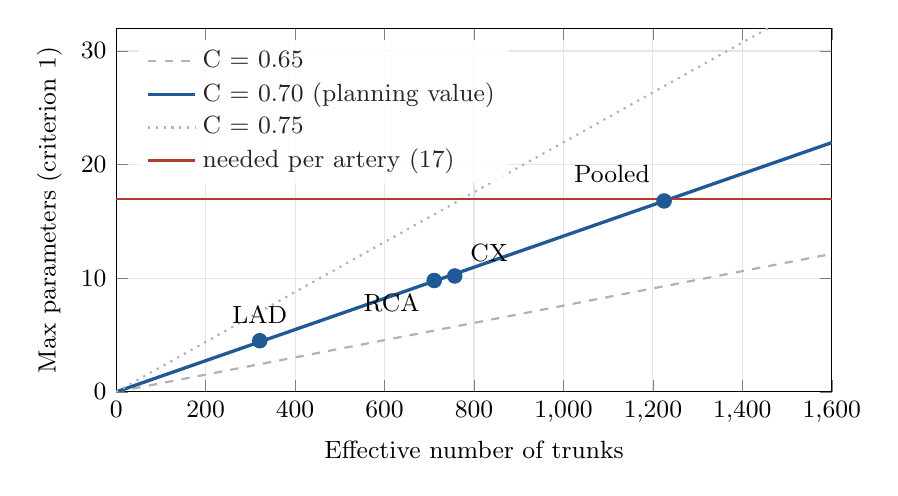
\begin{tikzpicture}
\begin{axis}[
  width=0.88\textwidth, height=6.2cm,
  xmin=0, xmax=1600, ymin=0, ymax=32,
  xlabel={Effective number of trunks}, ylabel={Max parameters (criterion 1)},
  legend pos=north west, legend cell align=left, legend style={font=\small, draw=none, fill=white, fill opacity=0.85},
  grid=major, grid style={gray!20}, tick label style={font=\small}, label style={font=\small},
]
\addplot[domain=0:1600, thick, gray!60, dashed] {0.00759*x};
\addlegendentry{C = 0.65}
\addplot[domain=0:1600, very thick, accent] {0.01371*x};
\addlegendentry{C = 0.70 (planning value)}
\addplot[domain=0:1600, thick, gray!60, dotted] {0.02196*x};
\addlegendentry{C = 0.75}
\addplot[domain=0:1600, thick, warn] {17};
\addlegendentry{needed per artery (17)}
\addplot[only marks, mark=*, mark size=2.6pt, accent] coordinates {(321,4.5) (757,10.2) (711,9.8) (1225,16.8)};
\node[font=\small, anchor=south] at (axis cs:321,5.2) {LAD};
\node[font=\small, anchor=north east] at (axis cs:700,9.4) {RCA};
\node[font=\small, anchor=south west] at (axis cs:770,10.6) {CX};
\node[font=\small, anchor=south east] at (axis cs:1215,17.6) {Pooled};
\end{axis}
\end{tikzpicture}
\end{center}

\subsection*{Worked example: the LAD}

321 plaque-free LADs, 139 developed plaque ($\phi = 0.43$). At C = 0.70, $R^2_{CS} = 0.119$, so
criterion~1 gives
\[
  P_{\max} = n\,(S-1)\ln\!\left(1-\tfrac{R^2_{CS}}{S}\right)
           = 321 \times (-0.1) \times \ln(1 - 0.132) \approx 4.5 .
\]
That is \textbf{4 parameters}, against 11 for the base model alone and 17 with geometry. In events
per parameter that is $139/4 \approx 35$, far stricter than the old ``10 EPV'' rule (which would
have allowed 13), because the signal is weak.

The LAD also fails criterion~3: estimating the average risk to $\pm 0.05$ needs at least
377 trunks, and there are 321.

\subsection*{How many trunks would one artery need?}

Solving criterion~1 for $n$ with $P = 17$ and C = 0.70:

\begin{center}
\begin{tabular}{lcccc}
\toprule
 & Needed trunks & Needed events & Available trunks & Shortfall \\
\midrule
LAD & $\approx 1\,200$ & $\approx 520$ &   321 & $\times 3.7$ \\
CX  & $\approx 1\,270$ & $\approx 460$ &   757 & $\times 1.7$ \\
RCA & $\approx 1\,230$ & $\approx 490$ &   711 & $\times 1.7$ \\
\bottomrule
\end{tabular}
\end{center}

\begin{warnbox}[What goes wrong if you fit them anyway]
\begin{itemize}\setlength\itemsep{2pt}
  \item Predicted risks are too extreme and need far more than 10\% shrinkage (miscalibration).
  \item The apparent C-statistic is optimistic and will not hold in new patients.
  \item A test of the 6-df geometry block is badly underpowered, so ``no added value'' means
        nothing, and a positive result is likely to be noise.
  \item Three separate geometry tests need a multiple-testing correction, which costs power again.
\end{itemize}
\end{warnbox}

\section{Why pooling helps, and its limits}

One model on all three arteries spends the base-model parameters \emph{once} instead of three
times. Risk factors, calcium and follow-up time act on the person, so their effects are estimated
from everyone. The arteries can still differ:
\begin{itemize}
  \item an \textbf{artery main effect} (2 df) gives each artery its own baseline risk;
  \item \textbf{geometry standardised within artery} puts ``high curvature'' on one scale for LAD,
        CX and RCA, so one shared slope per feature is meaningful;
  \item \textbf{1 to 3 prespecified artery $\times$ geometry interactions} test whether an effect
        really differs between arteries;
  \item \textbf{per-artery estimates} can be shown descriptively, with wide confidence intervals.
\end{itemize}

Even pooled, the budget is tight: 16 parameters at C = 0.70 against 19 needed. It fits at
C $\approx$ 0.72 or above, which is plausible given that calcium alone reaches 0.70. Otherwise,
trim the model, for example by reducing the geometry block to 3 to 4 features, or use
penalisation (ridge).

\section{Caveats}

\begin{itemize}
  \item \textbf{Proxy numbers.} The counts are vessel-level from \texttt{report.md}: they include
        side branches and do not apply the left-main rule. The chosen trunk design
        (\texttt{artery\_design()}, section 0 of \texttt{cgps\_stats.py}) was added after the report
        was generated. Re-run it to get the real counts; the LAD will most likely shrink further.
  \item \textbf{The unread half.} Only about 1\,020 of 2\,116 participants have baseline segment
        reads. If the other 1\,094 turn out to be genuinely plaque-free at baseline, every artery's
        budget roughly doubles or more. CX and RCA models might then become possible; the LAD would
        still be tight.
  \item \textbf{Clustering.} Dividing by the design effect is a heuristic, not part of Riley's
        published method; state it as an assumption.
  \item \textbf{Verify.} Use the \texttt{pmsampsize} package (R or Stata) with the final event
        fraction and an anticipated C, and report the inputs in the thesis.
\end{itemize}

\section*{References}
\begin{itemize}\setlength\itemsep{1pt}\small
  \item Riley RD et al. Minimum sample size for developing a multivariable prediction model:
        Part II -- binary and time-to-event outcomes. \emph{Stat Med} 2019;38:1276--96.
  \item Riley RD et al. Calculating the sample size required for developing a clinical prediction
        model. \emph{BMJ} 2020;368:m441.
  \item Riley RD, Van Calster B, Collins GS. A note on estimating the Cox--Snell $R^2$ from a
        reported C statistic (AUROC) to inform sample size calculations for developing a prediction
        model with a binary outcome. \emph{Stat Med} 2021;40:859--64.
  \item Lee SE et al. (PARADIGM) Clinical, imaging and laboratory predictors of plaque progression,
        2020 (clinical-only C = 0.684).
\end{itemize}

\end{document}
